\documentclass[11pt]{article}

\usepackage[margin=1in]{geometry}
\usepackage{booktabs}
\usepackage{graphicx}
\usepackage{amsmath}
\usepackage{amssymb}
\usepackage{hyperref}

\hypersetup{colorlinks=true, linkcolor=blue, urlcolor=blue}

\newcommand{\sep}{\texttt{x}}
\newcommand{\subj}[1]{\texttt{a\_#1}}
\newcommand{\obj}[1]{\texttt{b\_#1}}
\newcommand{\rel}[1]{\texttt{r\_#1}}
\newcommand{\fatt}[1]{\texttt{f\_#1}}
\newcommand{\gatt}[1]{\texttt{g\_#1}}
\newcommand{\Rsem}{R_{\mathrm{sem}}}
\newcommand{\Rrnd}{R_{\mathrm{rnd}}}

\title{Goal 2: A Frequent Relation Is Learned as Nonlinear}
\author{factual-recall-mechanisms}
\date{2026-07-03}

\begin{document}
\maketitle

\section{Claim and result in one paragraph}

A small transformer is trained for \textbf{exactly one epoch} on a synthetic corpus containing two relations with \emph{identical frequency statistics at every level} (same subjects, same 32 candidate objects, same number of triples, same number of occurrences per triple): a semantically supported relation $\Rsem$ and a random relation $\Rrnd$. At \emph{high} fact frequency ($F{=}64$ occurrences per triple) both relations are \emph{fully learned}: recall is $1.000$ on all 128 training triples for both, in all three seeds. Yet an affine map fitted by ordinary least-squares linear regression from subject representations to object representations identifies held-out targets at $0.891 \pm 0.056$ for $\Rsem$ and at $0.016 \pm 0.022$ ($=$ chance) for $\Rrnd$. The frequent random relation is therefore stored, but stored \emph{non-linearly}: no affine map over the same representations accounts for it, and it does not generalize (held-out recall at chance). Because the semantic relation at the very same frequency remains linear, the nonlinearity is attributable to the relation's semantics, not to its frequency; conversely, raising frequency from 1 to 64 occurrences never makes the random relation linear.

\section{Data}

\paragraph{Vocabulary (265 tokens).}
A separator \sep; two relation tokens \rel{0}, \rel{1}; 192 subject tokens $\subj{0},\dots,\subj{191}$; 32 object tokens $\obj{0},\dots,\obj{31}$; 32 attribute tokens $\fatt{0},\dots,\fatt{31}$; 6 attribute tokens $\gatt{0},\dots,\gatt{5}$.

\paragraph{Entities and attributes.}
Subject $\subj{i}$ carries the attribute pair $(f_{i \bmod 32},\ g_{\lfloor i/32\rfloor})$, so the 192 subjects realize each of the $32 \times 6$ attribute combinations exactly once. Object $\obj{j}$ carries $(f_{(j+3) \bmod 32},\ g_0)$.

\paragraph{Sentences.}
All training sentences have five tokens:
\begin{center}
\begin{tabular}{ll}
attribute sentence & \sep\ $\subj{i}$\ \fatt{p}\ \gatt{q}\ \sep \quad and \quad \sep\ $\obj{j}$\ \fatt{p}\ \gatt{q}\ \sep\\
relation triple & \sep\ $\subj{i}$\ $\rel{r}$\ $\obj{t}$\ \sep
\end{tabular}
\end{center}

\paragraph{Relations.}
\[
\Rsem(a_i) = b_{f(i)}, \qquad \Rrnd(a_i) = b_{\rho(i)},
\]
where $f(i) = i \bmod 32$ is the subject's own $f$-attribute index --- so the semantic target is the object whose $f$-attribute is the subject's, shifted by 3 --- and $\rho$ is a seed-dependent balanced random assignment onto the same 32 objects, independent of the attributes. Concrete example (seed 19): \subj{37} has attributes $(\fatt{5}, \gatt{1})$, so $\Rsem(\subj{37})=\obj{5}$, while $\Rrnd(\subj{37})=\obj{27}$; the training sentences are \sep\ \subj{37}\ \rel{0}\ \obj{5}\ \sep\ and \sep\ \subj{37}\ \rel{1}\ \obj{27}\ \sep.

\paragraph{Split and exact frequency matching.}
For every \fatt-value, 4 of its 6 subjects are \emph{trained} and 2 are \emph{held out} (128 trained, 64 held-out subjects; seed-dependent). $\rho$ is constructed balanced within both groups. Consequently, under \emph{both} relations: every trained subject occurs in exactly one triple per relation; every object is the target of exactly 4 trained and 2 held-out subjects; both relations contribute exactly 128 training triples, each repeated the same number of times ($F$). The two relations are indistinguishable by any frequency statistic; only the assignment semantics differ. Held-out subjects appear in attribute sentences but never in any relation triple. These invariants are asserted by \texttt{tests/test\_linear\_shift.py}.

\section{Model and training}

\begin{center}
\begin{tabular}{ll}
\toprule
Model & causal transformer, 1 layer, hidden 64, 4 heads, context 8\\
Embeddings & input and output embeddings untied; all weights $\mathcal{N}(0, 0.02^2)$\\
 & \textbf{no} attribute-based initialization; nothing frozen; no loss reweighting\\
Parameters & 84{,}288\\
Corpus & every attribute sentence $\times A{=}128$ ($= 28{,}672$ sentences)\\
 & $+$ 128 triples per relation, each $\times F$ ($F \in \{1,4,16,64\}$)\\
Training & \textbf{exactly one epoch}: a single pass over the shuffled corpus\\
Steps & 452 ($F{=}1$) to 704 ($F{=}64$) steps at batch size 64\\
Objective & unweighted next-token cross-entropy on all positions\\
Optimizer & AdamW, constant LR $10^{-3}$ after 5 linear warmup steps,\\
 & weight decay 0, gradient clip 1.0\\
Seeds & 19, 31, 47 (control data assignment, initialization, and data order)\\
\bottomrule
\end{tabular}
\end{center}

Note that ``frequent'' here means frequent within a single epoch: at $F{=}64$ the corpus contains each triple 64 times, but the model still passes over the corpus exactly once.

\section{The metric}

A single analysis metric is used, as an operationalization of ``the relation is an affine transformation'':

\begin{quote}
Fit $\hat W, \hat b$ by ordinary least-squares linear regression from the subject's \emph{input embedding} $s_i \in \mathbb{R}^{64}$ to the target object's \emph{output embedding} (unembedding row) $o_{R(i)} \in \mathbb{R}^{64}$, using the 128 trained pairs. For each of the 64 held-out subjects, predict $\hat W s_j + \hat b$ and select the nearest object row by cosine similarity among all 32 objects. Report the fraction of held-out subjects for which the selected object is $R(j)$. Chance is $1/32 \approx 0.03$.
\end{quote}

For every subject exactly one object is correct under each relation, so no top-$k$ metrics are needed or used. In addition, one \emph{learning check} (not an analysis metric) is recorded: greedy next-token recall of the model on prompts \sep\ $\subj{i}$\ $\rel{r}$, for trained and held-out subjects. For the claim ``learned as nonlinear'' this check is essential: it establishes that the relation \emph{is} stored.

\section{Results}

\begin{table}[h]
\centering
\begin{tabular}{rcccccc}
\toprule
 & \multicolumn{2}{c}{probe accuracy (held-out)} & \multicolumn{2}{c}{recall (trained)} & \multicolumn{2}{c}{recall (held-out)}\\
$F$ & $\Rsem$ & $\Rrnd$ & $\Rsem$ & $\Rrnd$ & $\Rsem$ & $\Rrnd$\\
\midrule
1  & $1.000 \pm .000$ & $.031 \pm .013$ & .029 & .010 & .016 & .010\\
4  & $1.000 \pm .000$ & $.016 \pm .013$ & .055 & .034 & .057 & .031\\
16 & $0.990 \pm .007$ & $.036 \pm .007$ & .672 & .167 & .635 & .031\\
\textbf{64} & $0.891 \pm .056$ & $\mathbf{.016 \pm .022}$ & \textbf{1.000} & \textbf{1.000} & .995 & \textbf{.031}\\
\bottomrule
\end{tabular}
\caption{Mean $\pm$ sd over seeds 19/31/47, at $A{=}128$ attribute-sentence occurrences. $F$ is the number of occurrences of each of the 128 triples per relation. Recall columns are the learning check. The headline cell is $F{=}64$: both relations are fully stored (recall 1.000), but only $\Rsem$ admits an affine map.}
\label{tab:goal2}
\end{table}

\begin{figure}[h]
\centering
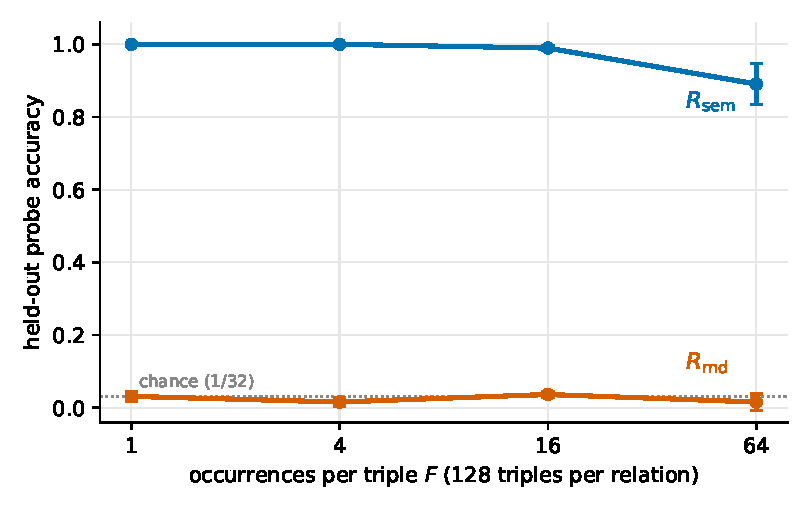
\includegraphics[width=0.65\textwidth]{figures/linear_shift_fsweep.pdf}
\caption{Held-out probe accuracy vs.\ occurrences per triple, for the two frequency-matched relations. The random relation is never linear, at any frequency; the semantic relation is linear at every frequency, with slight erosion at $F{=}64$.}
\label{fig:fsweep}
\end{figure}

\paragraph{Finding 1: a fully learned frequent relation with no linear structure ($F{=}64$).}
At 64 occurrences per triple, $\Rrnd$ reaches perfect recall of all 128 training triples --- the relation is fully stored --- while the affine probe remains at chance ($0.016 \pm 0.022$) and held-out recall is at chance ($.031$). The storage is a non-linear, non-generalizing memorization.

\paragraph{Finding 2: the nonlinearity is due to semantics, not frequency.}
$\Rsem$, trained in the same model from data with \emph{identical} frequency statistics, is equally fully stored (recall $1.000$) but linear (probe $0.891 \pm 0.056$) and generalizing (held-out recall $.995$). Conversely, increasing the frequency of $\Rrnd$ from 1 to 64 occurrences never produces linear structure (Fig.~\ref{fig:fsweep}): frequency determines only \emph{whether} the random relation gets stored (recall $.010 \rightarrow 1.000$), never \emph{in what format}.

\paragraph{Finding 3: high frequency slightly erodes the linear format of the semantic relation.}
$\Rsem$'s probe declines from $1.000$ ($F \le 4$) to $0.891 \pm .056$ ($F{=}64$), consistent with high-frequency memorization beginning to compete with the linear solution, while remaining far from the random relation's chance level.

\section{What this does and does not show}

\begin{itemize}
  \item \textbf{Shown:} a frequent relation can be fully learned and stored non-linearly (no affine map over the representations accounts for it, and it does not generalize); with frequency exactly matched, storage format is decided by semantics.
  \item \textbf{Qualification:} ``frequent $\Rightarrow$ nonlinear'' holds for the relation without attribute support. Frequency alone does not force nonlinearity: the frequent \emph{semantic} relation remains largely linear (with mild erosion at $F{=}64$). The precise claim supported is: at matched high frequency, an attribute-supported relation is stored linearly and an unsupported one non-linearly.
  \item \textbf{Superseded:} earlier drafts' high-frequency results used attribute-initialized embeddings (\texttt{structured\_embedding\_init}), targeted-row updates, and top-$k$ metrics; they are replaced by the present end-to-end setup with a single OLS metric.
\end{itemize}

\section{Reproduction}

Implementation: \texttt{experiments/factual\_recall/linear\_shift.py} (self-contained). Design invariants: \texttt{experiments/tests/test\_linear\_shift.py}. From \texttt{experiments/}:

\begin{small}
\begin{verbatim}
# Table 1 / Figure: one seed per command (19, 31, 47), ~1 min each on one GPU
uv run python -m factual_recall.linear_shift --world category --probe embedding \
  --seeds 19 --k-values 0,128 --occurrences 1,4,16,64 --attr-repeats 128 \
  --device cuda --output-dir factual_recall/results/final_category_seed19

# Aggregation/figures: factual_recall/results/final_summary/
uv run pytest tests/test_linear_shift.py -q
\end{verbatim}
\end{small}

Raw per-run metrics (including probe $R^2$/cosine and losses) are in \texttt{factual\_recall/results/final\_category\_*/linear\_shift\_metrics.json}. The companion document \texttt{goal1\_infrequent\_relation\_linear.pdf} covers the infrequent/linear claim on the same runs.

\end{document}
